%\VignetteIndexEntry{Partially Observed Boolean Dynamical Systems}
\documentclass[a4paper]{article}



\title{BoolFilter Package Vignette}
\author{Levi D. McClenny, Mahdi Imani, Ulisses Braga-Neto\\
        Dept. of Electrical and Computer Engineering\\
  	Texas A\&M University - College Station, TX\\
		\texttt{levimcclenny@tamu.edu, m.imani88@tamu.edu, ulisses@tamu.edu}}  %\texttt formats the text to a typewriter style font
\date{\today}  %\today is replaced with the current date


\usepackage{fancyhdr}


\usepackage{a4wide}

\usepackage{graphicx}
%\usepackage{amsmath}
\usepackage{hyperref}
\usepackage{amsmath,amssymb,amsthm,mathrsfs}
\usepackage{cite}
\usepackage{graphicx}
%\usepackage{fullpage}
\usepackage{amsmath}
\usepackage{pbox}
\usepackage{commath}
\usepackage{booktabs,caption}
\usepackage{multirow}
%\usepackage{kbordermatrix}
%\usepackage{fancyhdr}
\usepackage{lastpage}
\usepackage{float}
%\usepackage{pgfplots}

\usepackage{listings}
\lstset{breaklines=true, breakautoindent=false, breakindent=0pt, columns=fullflexible,keepspaces=true, basicstyle=\small\ttfamily}

\setlength{\parindent}{0em}
\setlength{\parskip}{0.2em}

\newcommand{\sbs}{\substack}
\newcommand{\bc}{\begin{center}}
\newcommand{\ec}{\end{center}}
\newcommand{\bi}{\begin{itemize}}
\newcommand{\ei}{\end{itemize}}
\newcommand{\ba}{\begin{array}}
\newcommand{\ea}{\end{array}}
\newcommand{\bal}{\begin{aligned}}
\newcommand{\eal}{\end{aligned}}
\newcommand{\beq}{\begin{equation}}
\newcommand{\eeq}{\end{equation}}
\newcommand{\bcs}{\begin{cases}}
\newcommand{\ecs}{\end{cases}}
\newcommand{\beqa}{\begin{eqnarray}}
\newcommand{\eeqa}{\end{eqnarray}}
\newcommand{\nn}{\nonumber}
\newtheorem{thm}{Theorem}
\newcommand{\argmax}{\operatornamewithlimits{argmax}}

\theoremstyle{plain}
\newtheorem{theorem}{Theorem}
\newtheorem{lemma}[theorem]{Lemma}
\newtheorem{proposition}[theorem]{Proposition}
\theoremstyle{definition}
\newtheorem{definition}[theorem]{Definition}
\newtheorem{problem}[theorem]{Problem}
\theoremstyle{remark}
\newtheorem{remark}[theorem]{Remark}

\def\prf{\noindent{\sc Proof}.\ }
\def\qed{Q.E.D. \vspace{1ex}}
\newcommand{\bprop}{\begin{proposition}}                                                                    
\newcommand{\eprop}{\end{proposition}}                                                                      

\def\bibdir{/Users/ulisses/doc/bib}

% Definitions
\def\rt{\rightarrow}
\def\Xk{{\bf X}_k}
\def\Zk{{\bf Z}_k}
\def\xk{{\bf x}_k}
\def\w{{\bf w}}
\def\M{{\bf M}}
\def\N{{\bf \textit{N}}}
\def\Tky{{T}_k{\bf (y)}}
\def\Yk{{\bf Y}_k}
\def\f{{\bf{f}}}
\def\v{{\bf{v}}}
%\def\uk{{\bf u}_k}
\def\uk1{{\bf{u}}_{k-1}}
\def\xone{{\bf{x}}_{1}}
\def\xzero{{\bf{x}}_{0}}
\def\Xkm{{\bf X}_{k-1}}
\def\Zkm{{\bf Z}_{k-1}}
\def\xkm{{\bf x}_{k-1}}
\def\h{{\bf{h}}}
\def\nk{{\bf n}_k}
\def\nkp{{\bf n}_{k+1}}
\def\vk{{\bf v}_k}
\def\uk{{\bf u}_k}
\def\rk{{\bf r}_k}
\def\nl{{\bf n}_{l}}
\def\vl{{\bf v}_l}
\def\xk{{\bf x}_k}
\def\yk{{\bf y}_k}
\def\hXk{{\bf \hat{X}}_k}
\def\hXkp{{\bf \hat{X}}_{k+1}}
\def\Xkp{{\bf X}_{k+1}}
\def\hWk{{\bf \hat{W}}_k}
\def\hWkm{{\bf \hat{W}}_{k-1}}
\def\hXkm{{\bf \hat{X}}_{k-1}}
\def\hfk{{\bf \hat{f}}_k}
\def\X{{\bf X}}
\def\Y{{\bf Y}}
\def\Z{{\bf Z}}
\def\Yon{{\bf Y}_1}
\def\etk{{\mbox{\boldmath $\eta$}_k}}
\def\mse{{\rm MSE}}
\def\msec{{\rm MSE}}
\def\x{{\bf x}}
\def\y{{\bf y}}
\def\yon{{\bf y}_1}
\def\Pik{{\bf \Pi}_{k|k}}
\def\Pikm{{\bf \Pi}_{k|k-1}}
\def\Pikmm{{\bf \Pi}_{k-1|k-1}}
\def\Ykm{{\bf Y}_{k-1}}
\def\Piz{{\bf \Pi}_{0|0}}
\def\PI{{\bf \Pi}}
\def\Xz{{\bf X}_0}
\def\xz{{\bf x}_0}
\def\Wz{{\bf W}_0}
\def\Mk{{M_k}}
\def\Tk{{T_k}}
\def\Mon{{M_1}}
\def\Ton{{T_1}}
\def\Ck{{C_k}}
\def\btk{{\mbox{\boldmath $\beta$}_k}}
\def\bt{{\mbox{\boldmath $\beta$}}}
\def\bb{{\mbox{\boldmath $b$}}}
\def\atk{{\mbox{\boldmath $\alpha$}_k}}
\def\alk{{\mbox{\boldmath $\alpha$}_k}}
\def\YN{{\bf Y}_N}
\def\Wk{{\bf W}_k}
\def\Wl{{\bf W}_l}
\def\Wkm{{\bf W}_{k-1}}
\def\etak{\eta_k}
\def\Sb{\bf S}
\def\obsplus{\diamondplus}
\def\vk{{\bf v}_k}
\def\vkm{{\bf v}_{k-1}}
\newcommand{\argmin}{\operatornamewithlimits{argmin}}


\widowpenalty=10000
\clubpenalty=10000

\hyphenation{me-thods pro-per-ties re-pre-sen-ta-tion}




\pagestyle{fancy}
\rhead{Partially-Observed Boolean Dynamical Systems}
\rfoot{R Package: BoolFilter}


\usepackage{Sweave}
\begin{document}
\Sconcordance{concordance:BoolFilter.tex:BoolFilter.Rnw:%
1 168 1 1 0 46 1 1 2 4 0 1 2 29 1 1 2 4 0 1 2 3 1 1 2 1 0 1 1 3 0 1 2 %
18 1 1 4 6 0 1 2 1 6 8 0 1 2 15 1 1 7 9 0 1 2 17 1 1 2 1 0 1 2 3 0 1 2 %
19 1 1 6 5 0 1 2 3 0 1 2 1 3 5 0 1 2 11 1 1 5 7 0 1 2 1 5 7 0 1 2 1 1 1 %
6 8 0 1 2 6 1 1 4 3 0 1 4 5 0 1 2 9 1 1 2 1 0 1 7 8 0 1 2 2 1 1 7 9 0 1 %
2 2 1 1 3 2 0 1 4 6 0 1 2 29 1 1 3 2 0 1 1 1 2 1 1 3 0 1 2 1 1 1 7 6 0 %
1 3 4 0 1 2 1 5 7 0 1 2 7 1}

\maketitle
\tableofcontents
\clearpage
\section{Introduction}


\indent The \texttt{BoolFilter} package provides tools for state estimation and inference of partially-observed Boolean dynamical systems. 
This package contains functions for simulating data, obtaining the optimal estimator in the presence of various observation noise models\cite{Brag:11}, applying the optimal MMSE filter and smoother\cite{ImanBrag:15b}, particle filter implementation of optimal filter~\cite{braga2013particle}, as well 
as means of parameter estimation and network inference\cite{ImanBrag:15a}.
\\[1em]
\indent \texttt{BoolFilter} was created explicitly to handle the latest tools developed for signal model of partially-observed Boolean dynamical system (POBDS).
This signal model, proposed in \cite{Brag:11}, was introduced to model dynamical systems containing Boolean variables observed indirectly through a noisy measurement process. This observation noise could be a result of instrumentation, incorrect thresholding, etc. 
\\[1em]
A characteristic signal model for the partially-observed Boolean dynamical system can be represented by the equations\cite{Brag:11}\cite{ImanBrag:16b}

\beq
\bal
  \Xk &\,=\, \f\left(\Xkm\right) \:\:\oplus\:\: \nk\quad \textrm{(state model)} \\[1ex]
  \Yk &\,=\, \h\left(\Xk,\vk\right) \quad \textrm{(observation model)}
\label{eq-sgnmodel}
\eal
\eeq

for $k=1,2,\ldots$. Here, $\nk \in \{0,1\}^d$ is Boolean transition noise,
``$\oplus$'' indicates component-wise
modulo-2 addition, and $\f: \{0,1\}^{d} \longrightarrow \{0,1\}^d$ is the network function,
whereas $\h$ is a
general function mapping the current state and observation noise $\vk$
into the measurement space. The
noise processes $\{\nk, \vk; k=1,2,\ldots\}$ are assumed to be
``white'' in the sense that the noises at distinct time points are
uncorrelated random variables.  
It is also assumed that the
noise processes are uncorrelated with each other and with the initial
 state $\Xz$.\\[1em]
Several tools for POBDSs have been developed in recent years such as the optimal filter and smoother based on the minimum mean square error (MMSE) criterion, called the Boolean Kalman Filter (BKF)~\cite{Brag:11} and Boolean Kalman Smoother (BKS)~\cite{ImanBrag:15b}, respectively. In addition, schemes for simultaneous state and parameter estimation, optimal filter in the case of correlated noise, network inference, fault detection, and control for POBDS were introduced in~\cite{ImanBrag:16b}\cite{LeviBrag:17}\cite{ImanBrag:15a}\cite{BahaBrag:15}\cite{ImanBrag:16a}\cite{ImanBrag:16c}.
\\[1em]
\texttt{BoolFilter} package is developed to make the latest developed tools for the POBDS accessible. First, the package can be installed from CRAN with the command 
 
\begin{Sinput}
> install.packages('BoolFilter')
\end{Sinput}

Once the package and its dependencies are fully installed, the package can be loaded into the workspace with the command 

\begin{Schunk}
\begin{Sinput}
> library('BoolFilter')
\end{Sinput}
\end{Schunk}
\section{Constructing a Boolean Network}
\textit{BoolFilter} relies on the package \textit{BoolNet} for describing Boolean Networks as input for its functions. This is done with a specific means of inputting a target gene, followed by its update rule\cite{mussel2015boolnet}. In order to create a Boolean Network, a text file must be created in the users current working directory with the transition rules in a specific format. For instance, the p53-MDM2 gene regulatory network is presented in Figure 1. The network contains 4 genes (ATM, p53, Wip1, Mdm2) and 1 input dna-dsb, which denotes the presence or absence of DNA double strand breaks.  This netwrok is shown below in figure 1:
\pagebreak
\begin{figure}[h]
\hfill
\begin{center}
\begin{minipage}{0.35\textwidth}
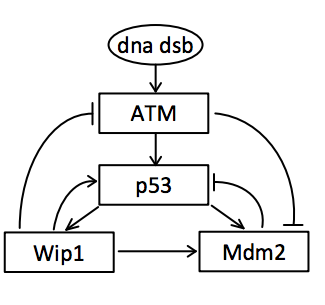
\includegraphics[width=1\textwidth]{Figure/p53.PNG}
\caption{p53-mdm2 Network}
\label{p53-mdm2 Network}
\end{minipage}
\end{center}
\end{figure}

One would create the network in a text file (named 'p53.txt', for instance, saved to the working directory) as follows:
\begin{verbatim}
targets, factors
ATM, (! Wip1 & 1)
p53, (ATM & ! Wip1 & ! Mdm2)
Wip1, p53
Mdm2, (!ATM & (p53 | Wip1)) | ( p53 & Wip1 )
\end{verbatim}

DNA\textunderscore dsb is an input to ATM. In the above Boolean network, DNA\textunderscore dsb is \textit{ON}. In order to toggle the input to \textit{OFF}, the first line would need to be changed to 

\begin{verbatim}
ATM, (! Wip1 & 0)
\end{verbatim}

Afterward, the network can be created into a Boolean Network class by utilizing functions in the \textit{BoolNet} package.
\begin{Schunk}
\begin{Sinput}
> p53net <- loadNetwork('p53.txt')
\end{Sinput}
\end{Schunk}
Again, this function is a part of \textit{BoolNet}, and creates an object of the type that \textit{BoolFilter} requires for its functionality. This allows for user specification of the genetic regulatory network. 

For simplicity, both p53 networks come included in the \textit{BoolFilter} package and can be loaded into the workspace using the command

\begin{Schunk}
\begin{Sinput}
> data(p53net_DNAdsb1) #DNA_dsb is ON
> data(p53net_DNAdsb0) #DNA_dsb is OFF
\end{Sinput}
\end{Schunk}
where ``p53-dnadsb0" and ``p53-dnadsb1" are referring to the p53-Mdm2 negative feedback loop regulatory network with external input 0 and 1 respectively.

In addition ``cellcycle" and ``melanoma" Boolean networks are available predefined in database of BoolNet and BoolFilter respectively. 

BoolNet also contains functions that allow for the reconstruction of Boolean networks from time series data, generating random networks with various connectivity parameters, or loading networks from SMBL or BioTapestry. More information on the various means of generating Boolean Networks with the BoolNet package can be found in the BoolNet Vignette at 
\url{https://cran.r-project.org/web/packages/BoolNet/vignettes/BoolNet_package_vignette.pdf}.

\section{Data Generation}

Network simulation takes a manually defined network and steps through the update rules, generating a time series of the genetic expression data of user-specified length. Process noise is assumed in the data generation, where the magnitude is a user defined parameter. For the data generation in \textit{BoolFilter}, we only considere i.i.d Bernoulli process noise. Two sets of state and measurement trajectories are created by BoolFilter.  
\\[1em]
Time series expression data can be generated using different observation models. This is useful in the sense that multiple observation noise models can potentially be found when analyzing genetic expression data. There exists a single parameter by which all the parameters for a given observation model can be input, called \textit{obsModel}. The order in which the parameters of observation models are input to the \textit{obsModel} parameter is outlined in the following sections. 
\\[1em]
Regardless of the observation model chosen to generate the data, the \textit{simulateNetwork} fuction will output a list consisting of the simulated state and measurement trajectories (called \textit{originalState} and \textit{observation}). 

\subsection{Bernoulli Observation Noise}

The first case will be Bernoulli observation noise. The intensity of Bernoulli observation noise is defined by parameter q (while p was the intensity of state transition process). The larger the noise parameter, the more noisy the measurements. Only one parameter value is required for Bernoulli observation noise, and \textit{BoolFilter} will throw an error if more than one parameter is input to a Bernoulli observation model. The following command creates state and observation trajectory with the length of n.data = 100, and intensity of Bernoulli state and process noise p = 0.05 and q = 0.02 respectively.

\begin{Schunk}
\begin{Sinput}
> data <- simulateNetwork(p53net_DNAdsb1, n.data = 100, p = .02,
+                       obsModel = list(type = 'Bernoulli', 
+                                       q = 0.05))
\end{Sinput}
\end{Schunk}

\begin{Schunk}
\begin{Sinput}
> #View both datasets overlayed
> plotTrajectory(data$X, 
+                labels = p53net_DNAdsb1$genes, 
+                dataset2 = data$Y, 
+                compare = TRUE)
\end{Sinput}
\end{Schunk}

\subsection{Gaussian Observation Noise}

BoolFilter is capable of generating data with Gaussian noise as well. In the event the user wants to create a Gaussian observation noise process, the parameters to the \textit{obsModel} parameter vector will be input in the following order:

\begin{verbatim}
mu0
sigma0
mu1
sigma1
\end{verbatim}


This model assumes that the Boolean states $\x = 0$ and $\x = 1$ are observed through Gaussian distributions $\xzero \sim \N$\textit{(mu0, sigma0)} and $\xone \sim \N$\textit{(mu1, sigma1)}, respectively, where {(mu0, sigma0)} and {(mu1, sigma1)} are pairs of the mean and standard deviation of the activated and inactivated conditions, respectively.


\begin{Schunk}
\begin{Sinput}
> data <- simulateNetwork(p53net_DNAdsb1, n.data = 100, p = 0.02,
+                       obsModel = list(type = 'Gaussian',
+                                       model = c(mu0 = 1, 
+                                              sigma0 = 2, 
+                                                 mu1 = 5, 
+                                             sigma1 = 2)))
\end{Sinput}
\end{Schunk}

This will generate a time series expression dataset with continuous entries,  in which the active and inactive genes are observed through $\xzero \sim \N$\textit{(1, 2)} and $\xone \sim \N$\textit{(5, 2)},

\subsection{Poisson Observation Noise}

\textit{BoolFilter} comes with a built-in Poisson observation model for modeling RNA sequencing data. Again, similar to the Gaussian observation model, the input parameters of obsModel in Poisson model are as follows:

\begin{verbatim}
s
mu
delta
\end{verbatim}

where \textit{s} is the sequencing depth, \textit{mu} is the baseline expression in inactivated state, and \textit{delta} is the differential expression.
\\[1em]
The \textit{delta} is a vector of the same magnitude as the number of Boolean variables where $delta_j$ denotes the effect of going from inactivated to activated state for $j$-th variable. In addition, \textit{mu} is a scaler usually between 0 and 1 characterizing the baseline level of expression, and sequencing depth \textit{s} is an instrument-dependent parameter. See \cite{ImanBrag:15b} and \cite{BahaBrag:15}, for more information about the range of different parameters.


\begin{Schunk}
\begin{Sinput}
> obsModel <- list(type = 'Poisson', s = 10.75, mu = 0.01, delta = c(2, 2, 2, 2))
> data <- simulateNetwork(p53net_DNAdsb1, n.data = 100, p = 0.02, obsModel)
\end{Sinput}
\end{Schunk}



\subsection{Negative-Binomial Observation Noise}

An additional observation model that can be used to model RNA-seq data is the Negative Binomial model. This model allows for the mean and variance to differ, unlike the Poisson distribution outlined in section 3.3. Similar to the Poisson model, the \textit{obsModel} parameter must be a list, however it adds another extra dispersion parameter vector referred to as \textit{phi}. The parameters should be input in the following order to obsModel:

\begin{verbatim}
s
mu
delta
phi
\end{verbatim}

Where \textit{s} is the sequencing depth, \textit{mu} is the baseline expression in inactivated state, and \textit{delta} is the differential expression, and \textit{phi} is the inverse dispersion.

Both \textit{delta} and \textit{phi} must be vectors of the same magnitude as the number of Boolean variables. This allows you to specify the observation model for each gene specifically, if so desired~\cite{ImanBrag:16b}. 
\\[1em]
Changing the \textit{type} variable to `NB' will cause the \textit{simulateNetwork} function to generate data from the negative binomial distribution as shown below: 

\begin{Schunk}
\begin{Sinput}
> obsModel <- list(type = 'NB', 
+                     s = 10.875, 
+                     mu = 0.01, 
+                  delta = c(3, 3, 3, 3), 
+                    phi = c(2, 2, 2, 2))
> data <- simulateNetwork(p53net_DNAdsb1, n.data = 100, p = 0.02, obsModel)
\end{Sinput}
\end{Schunk}
Data can be viewed in the following fashion, if desired:
\begin{Schunk}
\begin{Sinput}
> #display data without observation noise
> plotTrajectory(data$X, labels = p53net_DNAdsb1$genes)
\end{Sinput}
\end{Schunk}


\section{State Estimation of Partially-Observed Boolean Dynamical Systems}


\subsection{Boolean Kalman Filtering}

The Boolean Kalman Filtering algorithm is the optimal minimum mean-squared error (MMSE) estimator of a Partially-Observed Boolean Dynamical System\cite{Brag:11},\cite{ImanBrag:16b}. This algorithm estimates the state of the system recursively as new measurement arrives.
\\[1em]
Data from various sources can be fed into the BKF algorithm. Potential sources include RNA-seq, as well as user generated data outlined in section 3. The Boolean Kalman Filter implementation present in \textit{BoolFilter} is capable of handling all the observation noise discussed in section 3 regarding simulation - Bernoulli, Gaussian, Poisson, and Negative Binomial. The input to the BKF is handled in much the same way as the \textit{simulateNetwork} function, and assumes the user knows the distribution and parameters for the observation model.
\\[1em]
Use is as follows:
\begin{Schunk}
\begin{Sinput}
> #simulate bernoulli noise on p53 network
> data <- simulateNetwork(p53net_DNAdsb1, n.data = 100, p = .02,
+                       obsModel = list(type = 'Bernoulli', 
+                                       q = 0.02))
\end{Sinput}
\end{Schunk}
For this example, the p53 network was used for simplicity. Any network can be used, be it user specified, reconstructed, etc. 
\begin{Schunk}
\begin{Sinput}
> #run BKF algorithm on simulated data
> Results <- BKF(data$Y, p53net_DNAdsb1, p=0.02,
+                        obsModel = list(type = 'Bernoulli', 
+                                       q = 0.02))
\end{Sinput}
\end{Schunk}
The output, in this case labeled 'Results,' contains the estimated state, unnormalized posterior probability, as well as the conditional MSE at each time point. After performing the BKF and estimating states, the differences between the estimate and the original state trajectory can be viewed by plotting the trajectories of the genes using \textit{plotTrajectory} and comparing them as: 

\begin{Schunk}
\begin{Sinput}
> #plot the original and estimated trajectories on top of each other.
> plotTrajectory(data$X, 
+                labels = p53net_DNAdsb1$genes, 
+                dataset2 = Results$Xhat, 
+                compare = TRUE)
\end{Sinput}
\end{Schunk}


\subsection{Boolean Kalman Smoother}
In cases when the measurements are available offline, the optimal MMSE estimator of state is called Boolean Kalman Smoother\cite{ImanBrag:15b}. The method contains forward-backward process and can only be implemented on a batch data set. 
\\[1em]
The implementation is the same as the Boolean Kalman Filter:

\begin{Schunk}
\begin{Sinput}
> data <- simulateNetwork(p53net_DNAdsb1, n.genes = 100, p = 0.02,
+                       obsModel = list(type = 'Bernoulli',
+                                          q = 0.05))
> Results <- BKS(data$Y, p53net_DNAdsb1, p = 0.02,
+                       obsModel = list(type = 'Bernoulli',
+                                          q = 0.05))
\end{Sinput}
\end{Schunk}

It is again worth noting that the Boolean Kalman Filter algorithm is the optimal estimator for on-line process, whereas the Boolean Kalman Smoother is the optimal estimator for a given batch available data. 

\subsection{Particle Filter Implementation of BKF}
The Boolean Kalman Filter is the optimal MMSE estimator of a POBDS~\cite{Brag:11}. However, the computation of optimal filter becomes impractical for a large POBDS. This opens the floor for an approximation of the optimal estimator. In order to approximate a BKF, we implement a SIR-BKF  approach, outlined in \cite{braga2013particle}. 
\\[1em]
This approximation approach allows us to handle the issue of high dimensional networks in which the BKF approach can prove inefficient in the category of computational intensity. One such network is the 10-gene mammalian cell cycle network outlined in \cite{faure2006dynamical}
\\[1em]
Use of the SIR-BKF algorithm is outlined below, applied to the 10-gene Mammalian Cell Cycle network. First data is generated using the \textit{simulateNetwork()} function described in section 2:

\begin{Schunk}
\begin{Sinput}
> data(cellcycle)
> data <- simulateNetwork(cellcycle, n.data = 100, p = 0.02,
+                       obsModel = list(type = 'Gaussian',
+                                       model = c(mu0 = 1, 
+                                              sigma0 = 2, 
+                                                 mu1 = 5, 
+                                              sigma1 = 2)))
\end{Sinput}
\end{Schunk}

Then we apply the Particle Filter algorithm to obtain an approximation of the state variables through the observation noise:

\begin{Schunk}
\begin{Sinput}
> Results <- SIR_BKF(data$Y, N = 1000, alpha = 0.9, cellcycle, p = 0.02, 
+                          obsModel = list(type = 'Gaussian',
+                                       model = c(mu0 = 1, 
+                                              sigma0 = 2, 
+                                                 mu1 = 5, 
+                                              sigma1 = 2)))
\end{Sinput}
\end{Schunk}

The output 'Results' contains the estimated state and the conditional MSE at each time point. To compare the original and estimated state trajectories, one can use the following command:

\begin{Schunk}
\begin{Sinput}
> #compare the estimated and original state trajectories for selected Boolean variables
> VarPlot=c(1,2,5,7)
> plotTrajectory(data$X[VarPlot,], 
+                labels = cellcycle$genes[VarPlot], 
+                dataset2 = Results$Xhat[VarPlot,], 
+                compare = TRUE)
\end{Sinput}
\end{Schunk}

In the above code, the index \textit{c(1,4,5,7)} specifies the indices of Boolean variables to be plotted.

\section{Multiple Model Adaptive Estimation}

Suppose that the nonlinear signal model is
incompletely specified. For example, the relationship between Boolean variables may be only partially known, or the statistics of the noise
processes may need to be estimated. We assume that the missing
information can be coded into a finite-dimensional vector parameter $\Theta=\{\theta_1,...,\theta_M\}$. % where $\Theta$ is the parameter space. 
Assuming $P(\theta_i)$, for $i=1,...,M$, is the prior knowledge of $i$th model, the model selection is achieved by running a bank of BKFs running in parallel, one for
each candidate model. Setting initial probability of models as their prior ($p_0^i=P(\theta_i), \,i=1,...,M$), when measurement at time step $k$ appears, 
the probability of each model is updated recursively as follows:
\beq
p_k^i\,=\,\frac{||\bt_k^i||_1\,p_{k-1}^i}{\sum_{j=1}^M ||\bt_k^j||_1\,p_{k-1}^j}
\eeq
where $\bt_k^i$ denotes the unnormalized PDV at time $k$, computed at the update step of the BKF for model $\theta_i$. 

The process continues for different measurement recursively till the maximum
probability exceed a given threshold near $1$ ($\max_{i=1,...,M} p_k^i > t_s$). This leads to the following selected model:
\beq
\theta^* = \argmax_{i=1,...,M} p_k^i
\eeq
For more information about this method, refer to~\cite{ImanBrag:15a}.
\\[1em]
Two sources of unknown models can be modeled for implementation purposes:
\begin{enumerate}
\item Unknown network: User can define multiple networks as a possible network model to the system. 
\item Unknown process noise: Different possible intensities of Bernoulli process noise can be entered (as a vector) to the algorithm.
\end{enumerate}
The main algorithm is implemented as follows:
\begin{Schunk}
\begin{Sinput}
> #load potential networks
> data(p53net_DNAdsb0)
> data(p53net_DNAdsb1)
> net1 <- p53net_DNAdsb0
> net2 <- p53net_DNAdsb1
\end{Sinput}
\end{Schunk}

Once the networks have been identified, one can be simulated as follows:
\begin{Schunk}
\begin{Sinput}
> #define observation model
> observation = list(type = 'NB', 
+                       s = 10.875, 
+                      mu = 0.01, 
+                   delta = c(2, 2, 2, 2), 
+                     phi = c(3, 3, 3, 3))
> #simulate data using one of the networks and a given 'p'
> data <- simulateNetwork(net1, n.data = 100, p = 0.02, obsModel = observation)
\end{Sinput}
\end{Schunk}
The final step will be to call the MMAE function.
\begin{Schunk}
\begin{Sinput}
> #run MMAE to determine model selection and parameter estimation
> MMAE(data$Y, net = c("net1","net2"), p = c(0.02,0.1,0.15), threshold = 0.8, 
+                                                     Prior = NA,
+                                                     obsModel = observation)
\end{Sinput}
\end{Schunk}

Note that if the network or process noise intensity is known, one can only input them as their are to the algorithm. In addition, when the prior is not input to this function, uniform prior is considered for all models. 
\clearpage
\bibliographystyle{plain}
\bibliography{references}


\end{document}
